\documentclass[border = 0.2cm, 12pt]{standalone}
\usepackage{amsmath, amssymb, amsfonts}
\usepackage{color}
\usepackage{tikz, pgfplots}
\pgfplotsset{compat=newest}
\usetikzlibrary{shapes,snakes}
\tikzset{>=latex}
\usetikzlibrary{angles,quotes}
\usepackage{tkz-euclide}

\begin{document}

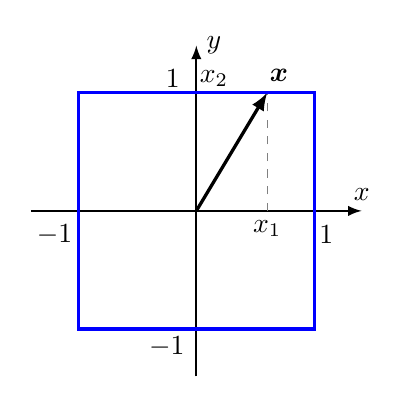
\begin{tikzpicture}[scale=1.5]

\draw[->,line width=0.7] (-1.4,0)--(1.4,0) node[above]{$x$};
\draw[->,line width=0.7] (0,-1.4)--(0,1.4) node[right]{$y$};

\draw[arrows=->, line width=1.2] (0,0)--(0.6,1);
\draw[dashed, color=gray, thin] (0.6,0)--(0.6,1);
\draw[color=blue, line width=1.2] (1,0)--(1,1)--(-1,1)--(-1,-1)--(1,-1)--(1,0);

\node at (0.6,-0.15) {$x_1$};
\node at (0.15,1.12) {$x_2$};
\node at (0.7,1.15) {$\boldsymbol{x}$};

\node at (1.1,-0.2) {$1$};
\node at (-1.2,-0.2) {$-1$};
\node at (-0.2,1.12) {$1$};
\node at (-0.25,-1.15) {$-1$};

\end{tikzpicture}

\end{document}